\section{Auswertung}
\label{sec:Auswertung}


Die Graphen wurden sowohl mit Matplotlib \cite{matplotlib} als auch NumPy \cite{numpy} erstellt. Die Fehlerrechnung wurde mithilfe von Uncertainties \cite{uncertainties} durchgeführt.

\subsection{Apparatekonstanten}
\label{sec:Apparatekonstanten}
Der Ausgang "Oscillator" liefert eine konstante Spannung von $\SI{11,5}{\volt}$.
Am Ausgang "Reference" lässt sich die Spannung regeln.

\subsection{Ausgangssignal ohne Rauschen}
\label{sec:oR}
\begin{figure}
\centering
\caption{Spannungsverläufe bei Phase $\Delta\phi$ ohne Tiefpassfilter}
\begin{minipage}{0.48\textwidth}
\center{$\Delta\phi=\SI{0}{\degree}$}
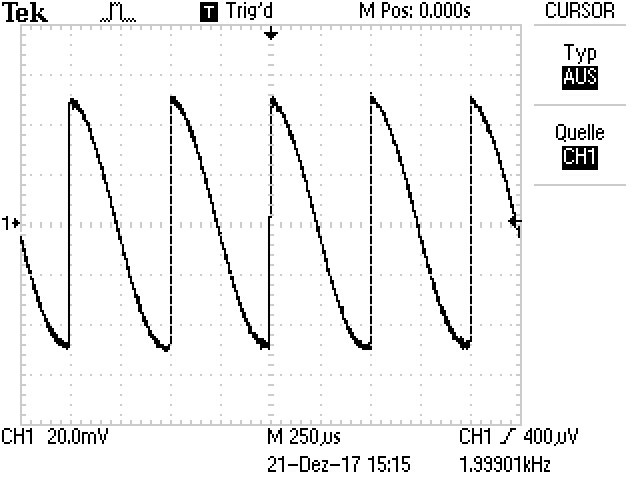
\includegraphics[scale=0.6]{content/images/00.jpg}
\end{minipage}
\begin{minipage}{0.48\textwidth}
\center{$\Delta\phi=\SI{45}{\degree}$}
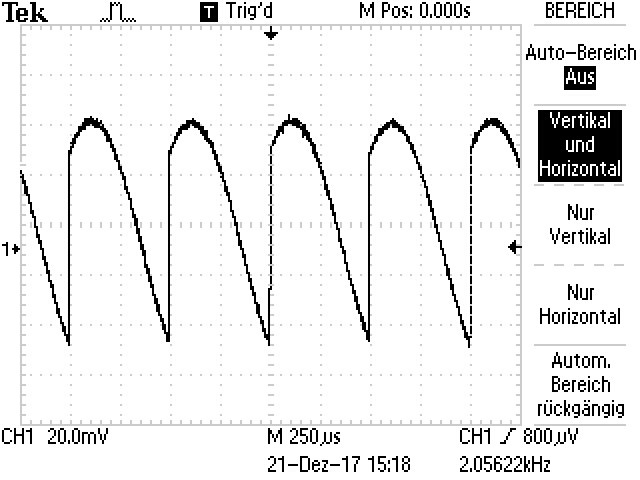
\includegraphics[scale=0.6]{content/images/45.jpg}
\end{minipage}
\begin{minipage}{0.48\textwidth}
\center{$\Delta\phi=\SI{90}{\degree}$}
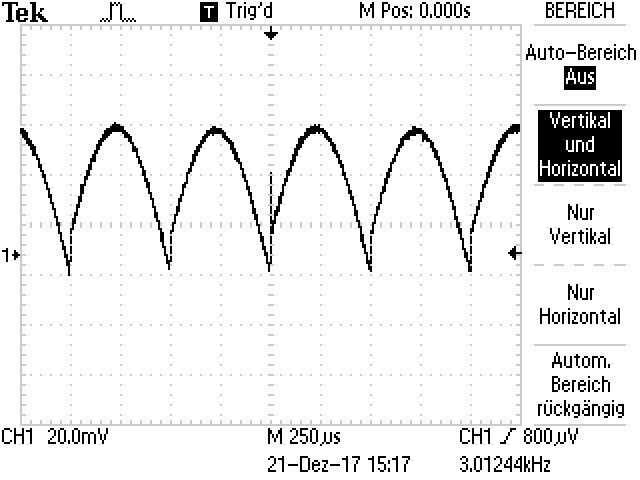
\includegraphics[scale=0.6]{content/images/90.jpg}
\end{minipage}
\begin{minipage}{0.48\textwidth}
\center{$\Delta\phi=\SI{180}{\degree}$}
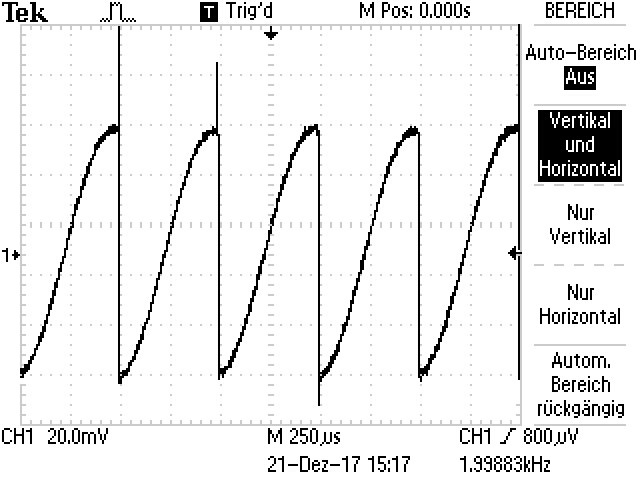
\includegraphics[scale=0.6]{content/images/180.jpg}
\end{minipage}
\center{$\Delta\phi=\SI{270}{\degree}$}
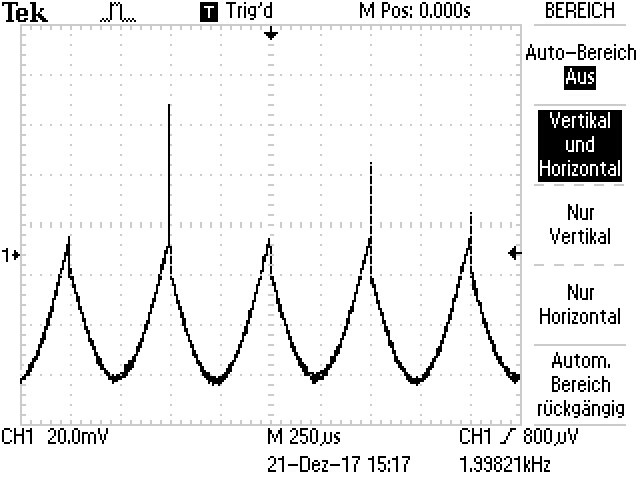
\includegraphics[scale=0.6]{content/images/270.jpg}
\label{fig:U}
\end{figure}
Die Signal-Spannung $U_.{Sig}$ am "Reference"-Ausgang wurde auf $\SI{10e-3}{\volt}$ bei $\SI{1000}{\hertz}$  und der Gain des "Pre-Amplifier" auf 2 eingestellt. Als Referenzspannung $U_.{ref}$ wird die in Abschnitt \ref{sec:Apparatekonstanten} genannte Spannung des "Oscillator"-Ausgangs verwendet und die Frequenz ebenfalls auf $\SI{1000}{\hertz}$ eingestellt. In Abbildung \ref{fig:U} sind die Spannungsverläufe für verschiedene Phasenverschiebungen $\Delta\phi$ abgebildet.
\begin{table}
	\centering
	\caption{Messwerte der Ausgangsspannung $U_.{out}$ nach dem Tiefpassfilter}
	\sisetup{table-format=1.2}
	\begin{tabular}{S[table-format=3.2] S[table-format=3.2]}
		\toprule
		{$\phi/\si{\degree}$}&{$U_.{out}/\si{\volt}$} \\
		\midrule
		45 & 2,52 \\
		90 & 4,08 \\
		105 & 4,16 \\
		135 & 3,32 \\
		150 & 2,16 \\
		180 & 0,44 \\
		225 & -2,68 \\
		270 & -4,08 \\
		315 & -3,24 \\
		360 & -0,45 \\
		\bottomrule
	\end{tabular}
	\label{tab:tab1}
\end{table}
\noindent Mit den Messwerten mit eingeschaltetem Tiefpassfilter aus Tabelle \ref{tab:tab1} wird die Regression
\begin{equation}
U_.{out}(\phi) = U_.{max}\cdot cos(f\cdot\phi+\phi_.0)\label{eq:Reg}
\end{equation}
durchgeführt:
\begin{align*}
U_.{max} &= \SI{4,13(5)}{\volt}
f 		 &= 17,5(1)e-3
\phi_.0  &= \SI{84(2)}{\degree}
\end{align*}
Mit Gleichung \eqref{eq:} ergibt sich für die Theoriekurve:
\begin{align*}
U_.{max,theo} &= \SI{12,7e-3}{\volt}
f_.{theo}	  &= 17,5e-3
\phi_.{0,theo}&= \SI{0}{\degree}
\end{align*}
Damit ergibt sich eine Abweichung von den experimentellen zu den theoretischen Werten von:
\begin{align*}
\Delta U_.{max} &= 32327\%
\Delta f		&= 0,00\%
\end{align*}
Die Graphen dazu sind in Abbildung \ref{fig:U2} zu sehen.
\begin{figure}
\centering
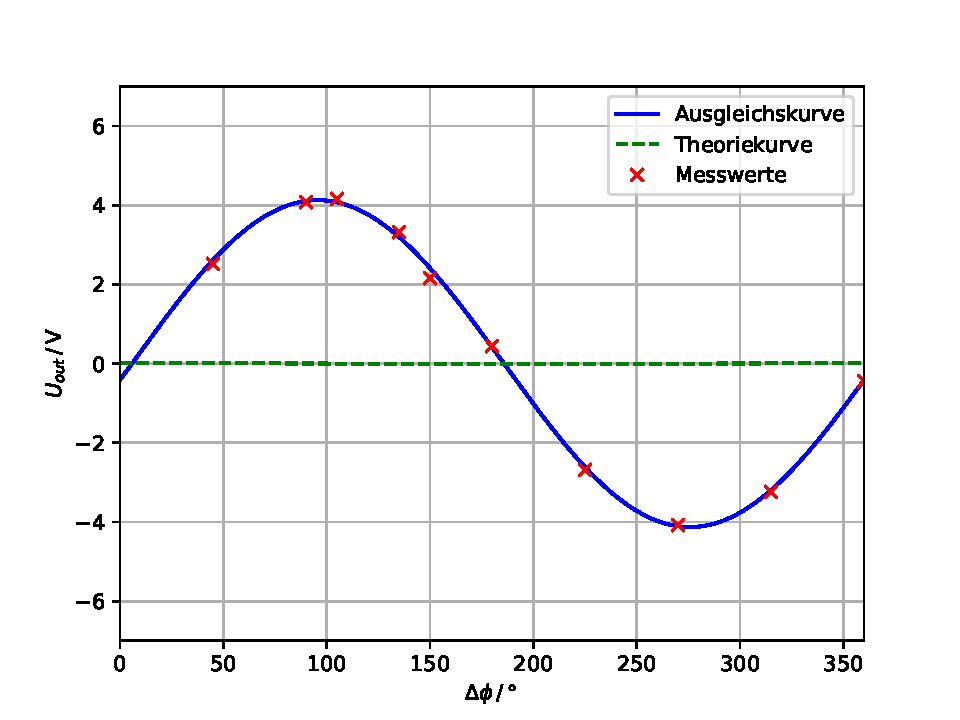
\includegraphics[scale=0.5]{content/images/plot.pdf}
\caption{Graphen der Messwerte mit Tiefpassfilter, ohne Noise-Schaltung}
\label{fig:U2}
\end{figure}
\subsection{Ausgangssignal mit Rauschen}
\label{sec:mR}
Es wurde die Noise-Schaltung auf $10^-3$ gestellt. Die Spannungsverläufe für verschiedene Phasendifferenzen in Abbildung \ref{fig:U3}
\begin{figure}
\centering
\caption{Spannungsverläufe bei Phase $\Delta\phi$ ohne Tiefpassfilter mit Noise-Schaltung}
\begin{minipage}{0.48\textwidth}
\center{$\Delta\phi=\SI{0}{\degree}$}
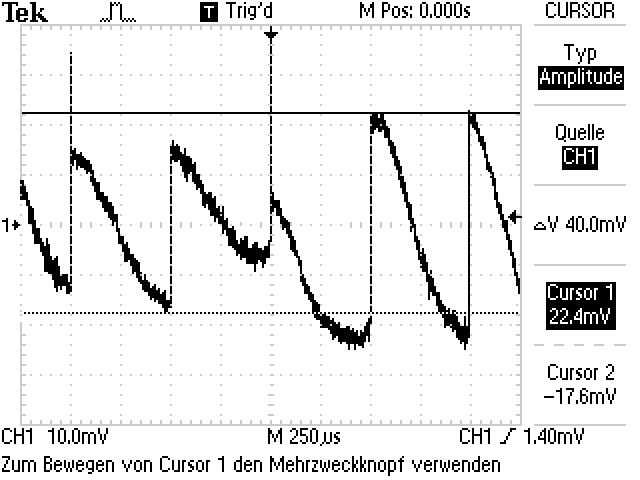
\includegraphics[scale=0.6]{content/images/noise0.jpg}
\end{minipage}
\begin{minipage}{0.48\textwidth}
\center{$\Delta\phi=\SI{45}{\degree}$}
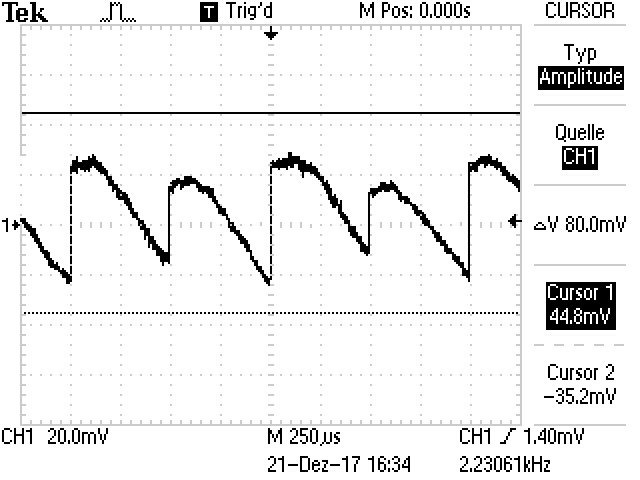
\includegraphics[scale=0.6]{content/images/noise45.jpg}
\end{minipage}
\begin{minipage}{0.48\textwidth}
\center{$\Delta\phi=\SI{90}{\degree}$}
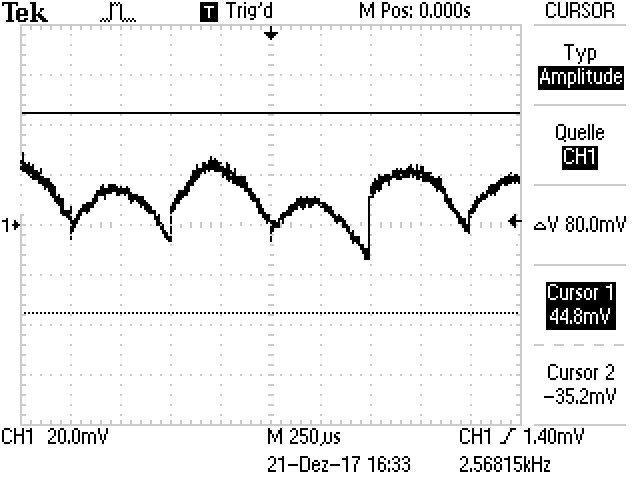
\includegraphics[scale=0.6]{content/images/noise90.jpg}
\end{minipage}
\begin{minipage}{0.48\textwidth}
\center{$\Delta\phi=\SI{180}{\degree}$}
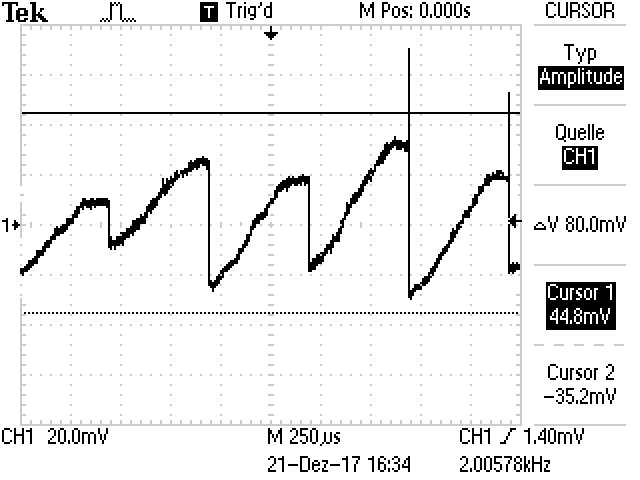
\includegraphics[scale=0.6]{content/images/noise180.jpg}
\end{minipage}
\center{$\Delta\phi=\SI{270}{\degree}$}
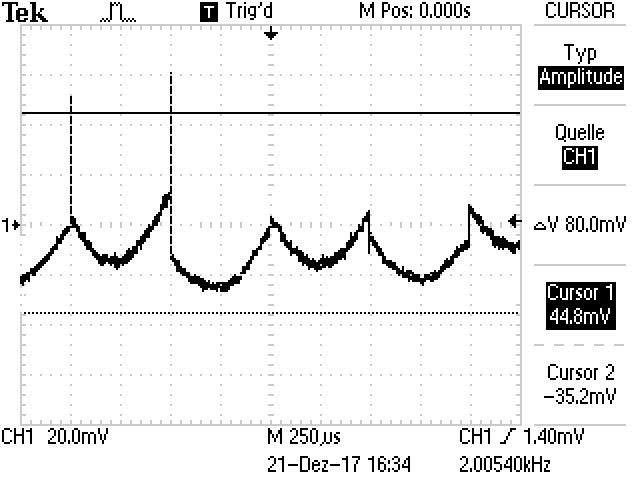
\includegraphics[scale=0.6]{content/images/noise270.jpg}
\label{fig:U3}
\end{figure}
\begin{table}
	\centering
	\caption{Messwerte der Ausgangsspannung $U_.{out}$ nach dem Tiefpassfilter mit Noise-Schaltung}
	\sisetup{table-format=1.2}
	\begin{tabular}{S[table-format=3.2] S[table-format=3.2]}
		\toprule
		{$\phi/\si[per-mode=reciprocal]{\degree}$}&{$U_.{out}/10^-3/\si[per-mode=reciprocal]{\volt}$} \\
		\midrule
		45 & 34,4 \\
		90 & 59,2 \\
		105 & 60,8 \\
		135 & 52,8 \\
		150 & 34,4 \\
		180 & 13,0 \\
		225 & -32,8 \\
		270 & -56,0 \\
		315 & -48,0 \\
		360 & -11,4 \\
		\bottomrule
	\end{tabular}
	\label{tab:tab2}
\end{table}
Die Messwerte nach Zuschalten des Tiefpassfilters und Erhöhung des Pre-Amplifier-Gains auf 10 sind in Tabelle \ref{tab:tab2} zu sehen. Damit wird wird die lineare Regression nach Gleichung \eqref{eq:Reg} durchgeführt.
Es ergeben sich:
\begin{align*}
U_.{max} &= \SI{5,9(1)e-2}{\volt}
f 		 &= 17,4(1)e-3
\phi_.0  &= \SI{84(2)}{\degree}
\end{align*}
Mit Gleichung \eqref{eq:} ergibt sich für die Theoriekurve:
\begin{align*}
U_.{max,theo} &= \SI{6,3e-2}{\volt}
f_.{theo}	  &= 17,5e-3
\phi_.{0,theo}&= \SI{0}{\degree}
\end{align*}
Damit ergeben sich die Abweichungen:
\begin{align*}
\Delta U_.{max} &= 6,79\%
\Delta f		&= 0,29\%
\end{align*}
Die Graphen dazu sind in Abbildung \ref{fig:U4} zu sehen.
\begin{figure}
\centering
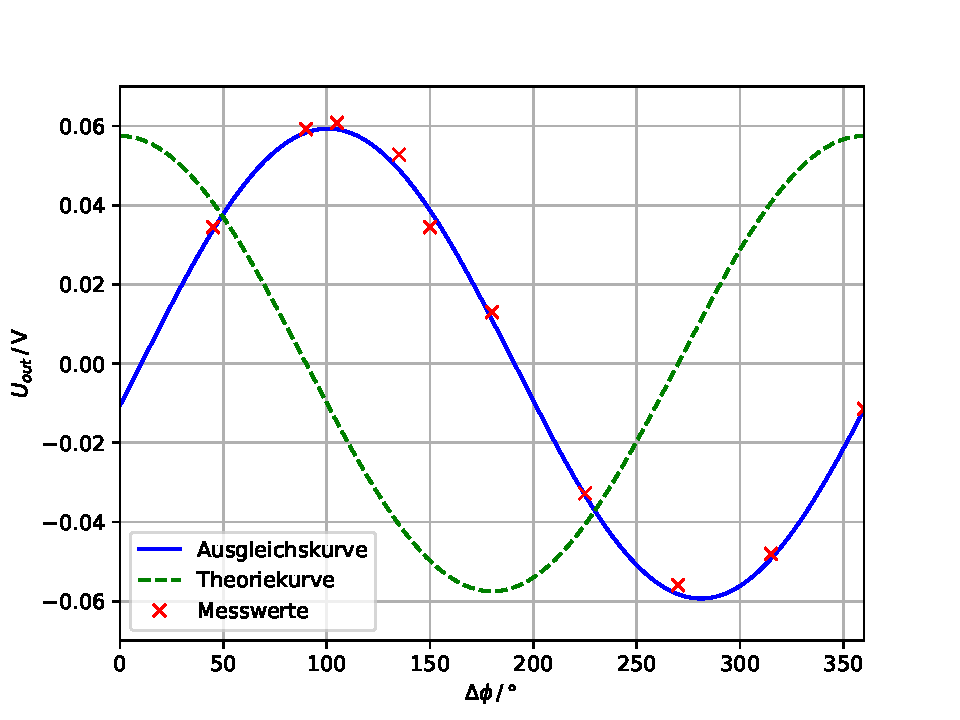
\includegraphics[scale=0.5]{content/images/plot2.pdf}
\caption{Graphen der Messwerte mit Tiefpassfilter, mit Noise-Schaltung}\label{fig:U4}
\end{figure}
\subsubsection{Leuchtdiode}
Die Pulsfrequenz der LED wurde auf $\SI{200}{\hertz}$ und die Verstärkung am Pre-Amplifier auf 50 eingestellt. Die gemessenen Werte der Spannung $U$ bei verschiedenen Abständen $r$ sind in Tabelle \ref{tab:tab3} zu sehen
\begin{table}
	\centering
	\caption{Messwerte der Ausgangsspannung $U_.{out}$ nach dem Tiefpassfilter mit Noise-Schaltung}
	\sisetup{table-format=1.2}
	\begin{tabular}{S[table-format=3.2] S[table-format=3.2]}
		\toprule
		{$r/10^2/\si[per-mode=reciprocal]{\metre}$}&{$U/\si[per-mode=reciprocal]{\volt}$} \\
		\midrule
		30 11,2 \\
		34 9,00 \\
		38 7,40 \\
		42 6,17 \\
		46 5,25 \\
		50 4,49 \\
		54 3,92 \\
		58 3,36 \\
		62 2,98 \\
		66 2,65 \\
		70 2,32 \\
		74 2,05 \\
		78 1,83 \\
		82 1,62 \\
		86 1,45 \\
		90 1,37 \\
		94 1,26 \\
		98 1,16 \\
		102 1,08 \\
		106 1,00 \\
		110 0,925 \\
		114 0,86 \\
		118 0,8 \\
		122 0,74 \\
		126 0,7 \\
		130 0,65 \\
		134 0,6 \\
		138 0,51 \\
		\bottomrule
	\end{tabular}
	\label{tab:tab3}
\end{table}
In Abbildung \ref{fig:U5} U gegen r aufgetragen.
\begin{figure}
\centering
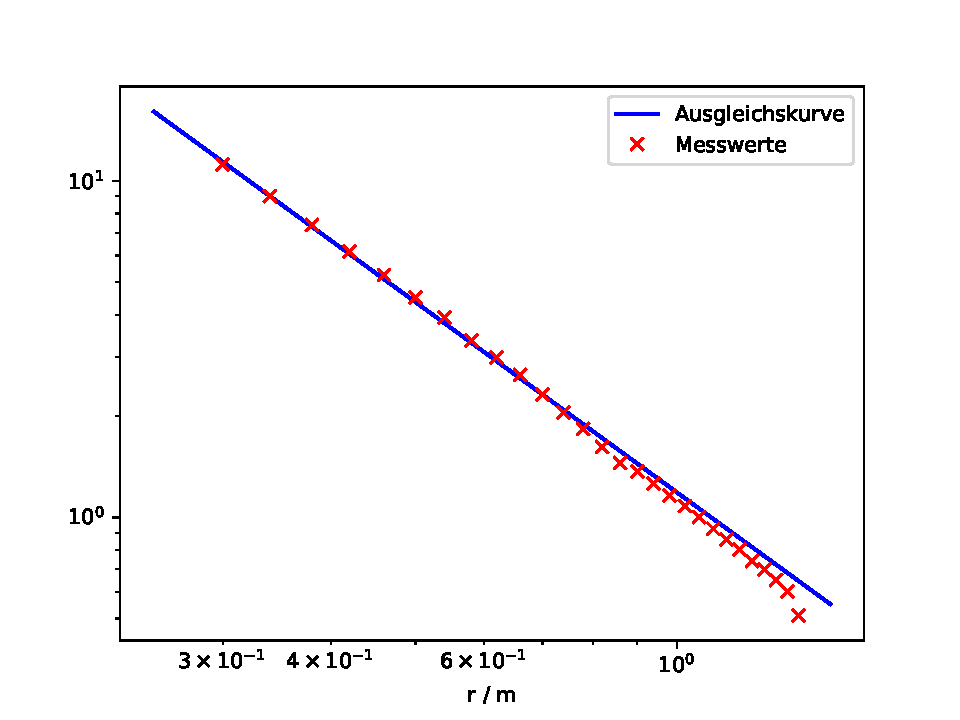
\includegraphics[scale=0.5]{content/images/plot3.pdf}
\caption{Logarithmische Darstellung des Verhaltens der Spannung bei zunehmendem Abstand der Leuchtdiode}\label{fig:U5}
\end{figure}
Mittels der Regression $U(r)=a\cdot r^{-b}$ ergibt sich
\[
b_.{gemessen}=1,88(2)
\]
Der theoretische Wert für $b$ liegt bei 
\[
b_.{theo}=2
\]
Somit beträgt die Abweichung
\[
\Delta b = 5,95 \%
\]